\section{简介}

D3.js(D3或Data-Driven Documents)是一个使用动态图形,基于数据操作文档的,进行数据可视化的JavaScript程序库。D3 帮助您通过使用 HTML、SVG 和 CSS 使数据栩栩如生,产生交互式的数据展示效果——分层条形图、动画树状图、力导向图、等高线、散点图……。 且D3 提供了现代浏览器的全部功能,无需将束缚在特定框架中,可以与Vue、React等结合使用,提供强大的可视化组件和数据驱动的 DOM 操作方法。目前最新版本的D3已经更新到了7.0版本(截止到2021年7月)。

D3 是一个开源项目,其源码托管于 GitHub,地址为\url{https://github.com/d3/d3},官网地址为\url{https://d3js.org/}。另外,官方的Wiki手册和推荐资源可在\url{https://github.com/d3/d3/wiki}中找到。

D3.js有这样一些特点:

\begin{enumerate}
    \item \textbf{使用 Web 标准:}D3 是一个非常强大的可视化工具,用于创建交互式数据可视化。它利用现代网络标准:SVG、HTML 和 CSS 来创建数据可视化。
    \item \textbf{数据驱动:}D3 是数据驱动的。它可以使用静态数据或从远程服务器以不同格式(如数组、对象、CSV、JSON、XML 等)获取数据来创建不同类型的图表。
    \item \textbf{DOM 操作:}D3 允许您根据数据操作文档对象模型 (DOM)。
    \item \textbf{数据驱动元素:}它使您的数据能够动态生成元素并将样式应用于元素,表格、图形等都支持。
    \item \textbf{动态属性:}D3 可以灵活地为其大部分功能提供动态属性。属性可以指定为数据的函数。这意味着您的数据可以驱动您的样式和属性。
    \item \textbf{可视化类型:}对于 D3,尽管没有标准的可视化格式,但它允许你自由发挥,创建 从HTML 表格到饼图、图形、条形图到地理空间地图等任何内容。
    \item \textbf{自定义可视化效果:}由于 D3 使用 Web 标准,因此您可以完全控制可视化功能。
    \item \textbf{交互和动画:}D3 通过 \verb|duration()|、\verb|delay()| 和\verb|ease()| 等函数为动画提供了很好的支持,能快速响应用户交互的需要。 
\end{enumerate}

如\figref{fig:example_population_pyramid}、\figref{fig:example_bubble_chart}、\figref{fig:example_circle_packing}、\figref{fig:example_stream_graph}中所示,这些都是用D3.js所绘制出的交互式数据可视化图表。

\begin{figure}[htbp]
    \centering
    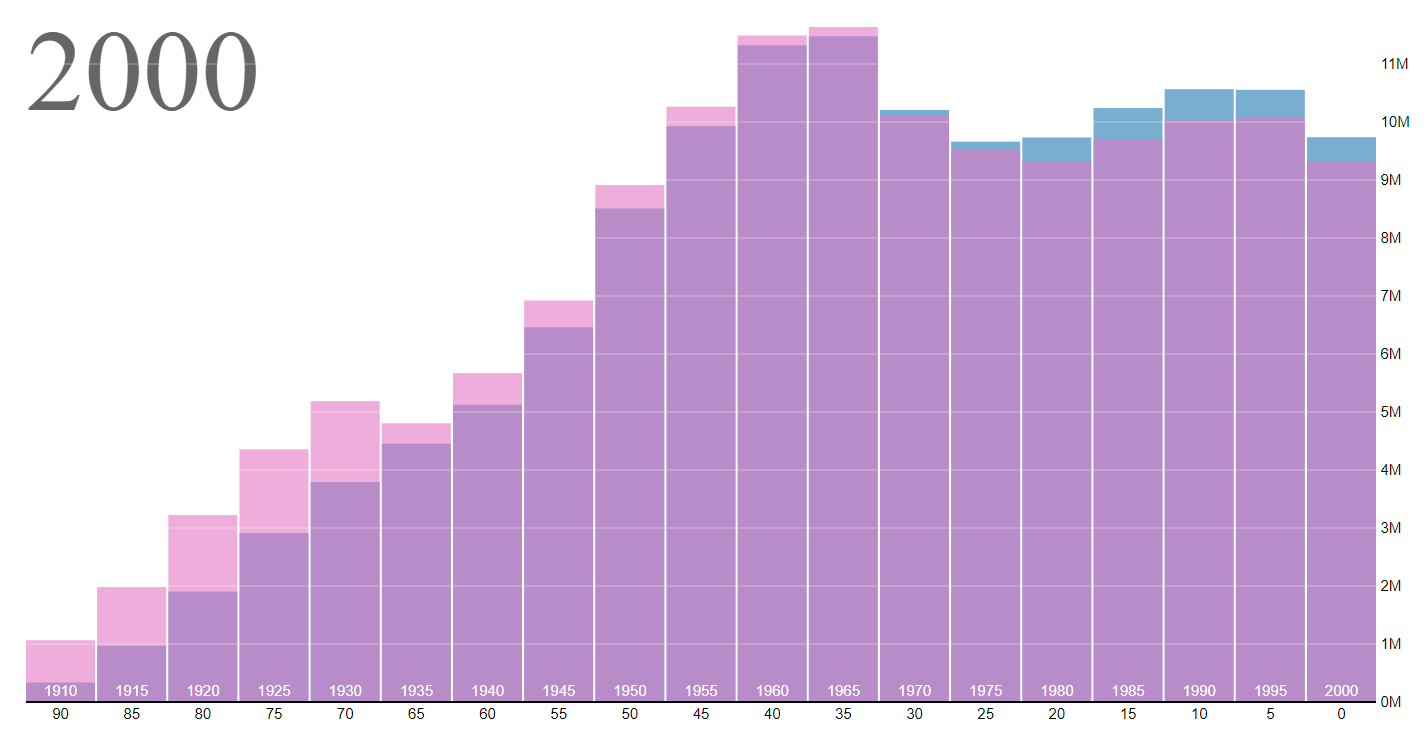
\includegraphics[width=0.8\textwidth]{figure/D3/example_population_pyramid.png}
    \caption{\textbf{示例条形图}}
    \label{fig:example_population_pyramid}
\end{figure}

\begin{figure}[htbp]
    \centering
    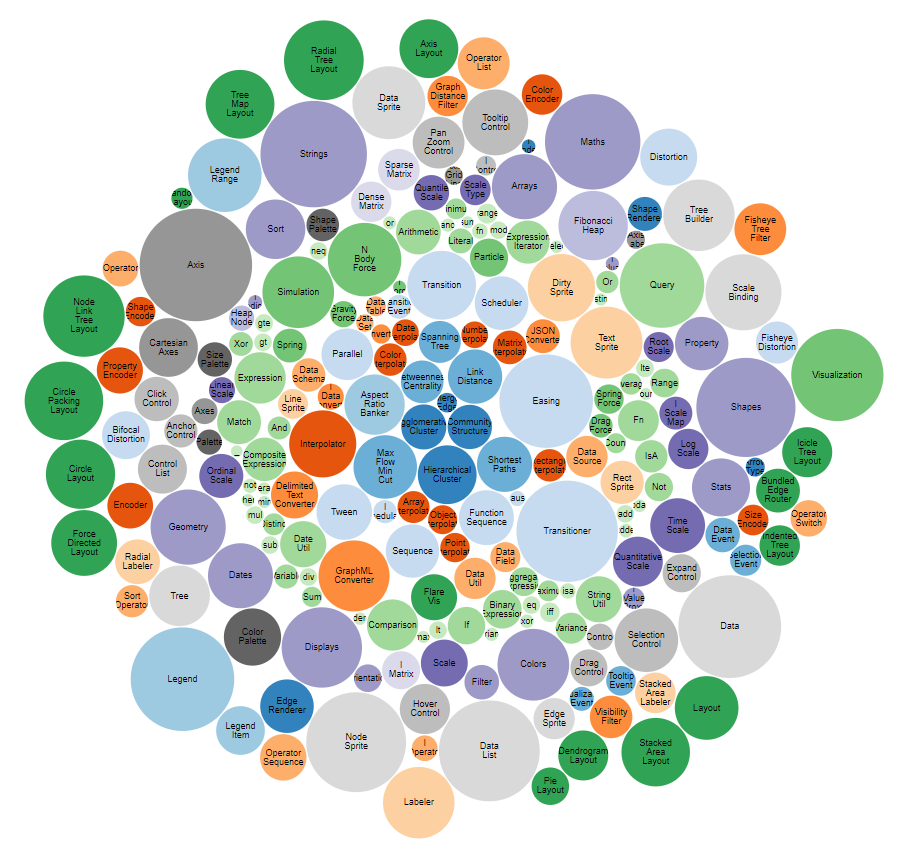
\includegraphics[width=0.8\textwidth]{figure/D3/example_bubble_chart.png}
    \caption{\textbf{示例气泡图}}
    \label{fig:example_bubble_chart}
\end{figure}

\begin{figure}[htbp]
    \centering
    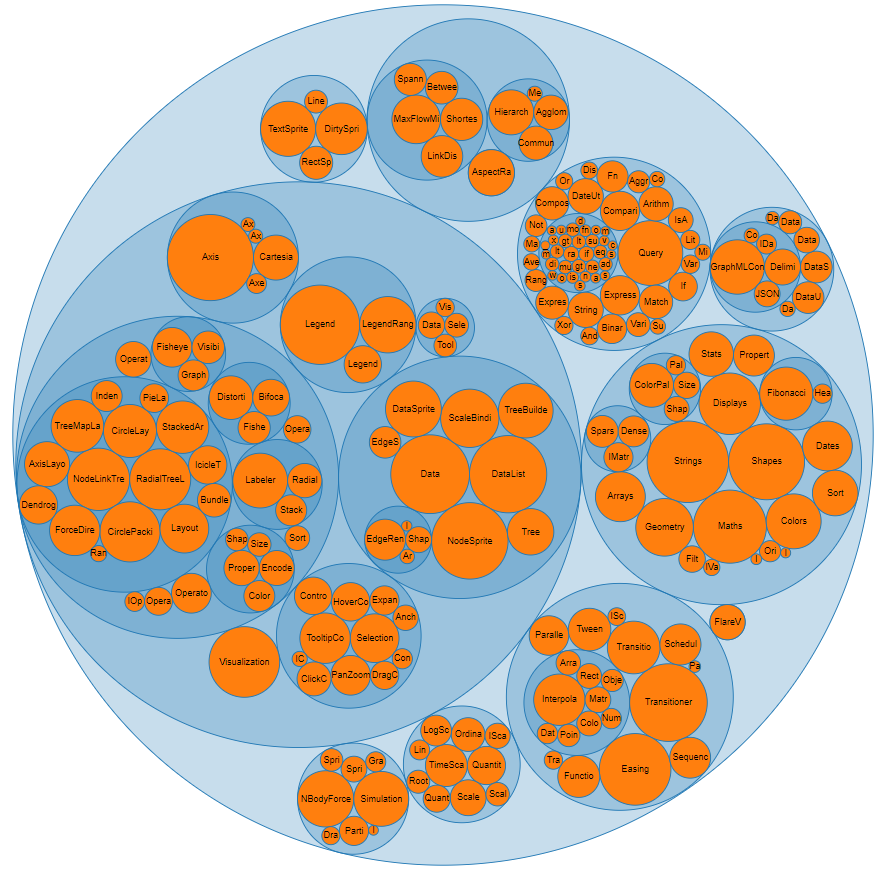
\includegraphics[width=0.8\textwidth]{figure/D3/example_circle_packing.png}
    \caption{\textbf{示例圈层图}}
    \label{fig:example_circle_packing}
\end{figure}



\begin{figure}[htbp]
    \centering
    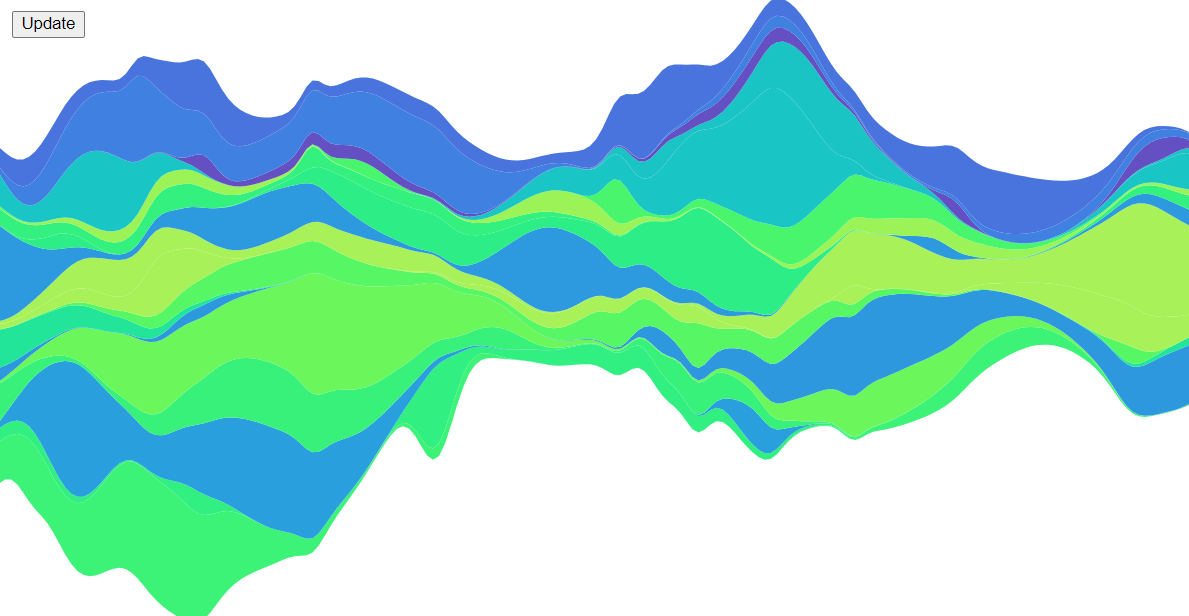
\includegraphics[width=0.8\textwidth]{figure/D3/example_stream_graph.png}
    \caption{\textbf{示例流图}}
    \label{fig:example_stream_graph}
\end{figure}


\section{安装}

D3 作为一个 JavaScript 函数库,其实并不是标题中所说的``安装'',更准确地说是``导入''。它只有单文件,在 HTML 中引用即可。有两种方法:

\textbf{方法一:}从官网处下载D3.js的压缩包文件并解压。

当前官网可下载到最新7.0.0版本的D3,链接为\url{https://registry.npmjs.org/d3/-/d3-7.0.0.tgz}。

解压后,在 HTML 中导入相关的 js 文件即可使用D3。( \verb|package/dist| 文件夹下的 \verb|d3.js| 或 \verb|d3.min.js|,其中含min的文件为压缩后版本)

\textbf{方法二:}直接通过网络上的D3地址,引用链接到HTML中。

\begin{minted}
[
frame=lines,
framesep=2mm,
baselinestretch=1.2,
fontsize=\footnotesize,
linenos
]{html}
<script src="https://d3js.org/d3.v7.min.js"></script>
\end{minted}

注意应用方法二时,需要保证使用D3时网络畅通。

注:本章节中所使用到的D3版本为7.0.0版本。

\section{预备知识和工具}

D3是作为JavaScript语言编写的程序库,常应用并展示于网页浏览器之中,故离不开制作网页相关的技术栈,主要包括了这样一些预备知识:

\begin{enumerate}
    \item HTML:超文本标记语言,用于设定网页的内容
    \item CSS:层叠样式表,用于设定网页的样式
    \item JavaScript:一种直译式脚本语言,用于设定网页的行为
    \item DOM:文档对象模型,用于修改文档的内容和结构
    \item SVG:可缩放矢量图形,用于绘制可视化的图形
\end{enumerate}

本章节对D3的应用不需要对这以上几个技术有很深的了解,大概知道其作用即可。我们会通过D3的案例简单地综合运用,重点则关注于D3的使用和操作上。

D3可以认为是一套含有可视化代码片段模板的程序库,操作D3的数据可视化应用还要通过编程写代码来实现。通常以制作网页的形式来呈现出D3可视化的数据。在此推荐使用几个制作网页时会用到的D3编程相关工具。

\begin{enumerate}
    \item 编辑器:Visual Studio Code(VS Code),微软出品的非常强大且流行的编辑器,在前端开发者中广泛使用。配合插件,开发体验非常好。
    \item 浏览器:Chrome、Firefox、Edge等主流浏览器均可。
\end{enumerate}